\input{../YKY-preamble.tex}
% \usepackage[no-math]{fontspec}
% \setmainfont[BoldFont=Alibaba_Sans_Regular.otf,ItalicFont=Alibaba_Sans_Light_Italic.otf]{Alibaba_Sans_Light.otf}

\usepackage[backend=biber]{biblatex}
\bibliography{../AGI-book}

\usepackage[active,tightpage]{preview}		% for continuous page(s)
\renewcommand{\PreviewBorder}{0.5cm}
\renewcommand{\thempfootnote}{\arabic{mpfootnote}}

\usepackage[absolute,overlay]{textpos}		% for page number on upper left corner

\usepackage{color}
% \usepackage{mathtools}
\usepackage[hyperfootnotes=false]{hyperref}

% \usepackage[backend=biber,style=numeric]{biblatex}
% \bibliography{../AGI-book}
% \renewcommand*{\bibfont}{\footnotesize}

\usetikzlibrary{shapes}
% \usepackage[export]{adjustbox}	% ??
\usepackage{verbatim} % for comments
% \usepackage{newtxtext,newtxmath}	% Times New Roman font

% \titleformat{\subsection}[hang]{\bfseries\large\color{blue}}{}{0pt}{} 
% \numberwithin{equation}{subsection}

\newcommand{\underdash}[1]{%
	\tikz[baseline=(toUnderline.base)]{
		\node[inner sep=1pt,outer sep=10pt] (toUnderline) {#1};
		\draw[dashed] ([yshift=-0pt]toUnderline.south west) -- ([yshift=-0pt]toUnderline.south east);
	}%
}%

\newcommand\reduline{\bgroup\markoverwith{\textcolor{red}{\rule[-0.5ex]{2pt}{0.4pt}}}\ULon}

%\DeclareSymbolFont{symbolsC}{U}{txsyc}{m}{n}
%\DeclareMathSymbol{\strictif}{\mathrel}{symbolsC}{74}
%\DeclareSymbolFont{AMSb}{U}{msb}{m}{n}
%\DeclareSymbolFontAlphabet{\mathbb}{AMSb}
%\setmathfont{lmroman17-regular.otf}
\DeclareMathOperator*{\argmin}{arg\,min}
\DeclareMathOperator*{\argmax}{arg\,max}

% \usepackage[most]{tcolorbox}
%\tcbset{on line, 
%	boxsep=4pt, left=0pt,right=0pt,top=0pt,bottom=0pt,
%	colframe=red,colback=pink,
%	highlight math style={enhanced}
%}
%\newcommand{\atom}{\vcenter{\hbox{\tcbox{....}}}}

\let\oldtextbf\textbf
\renewcommand{\textbf}[1]{\textcolor{blue}{\oldtextbf{#1}}}

\newcommand{\logic}[1]{{\color{violet}{\textit{#1}}}}
\newcommand{\underconst}{\includegraphics[scale=0.5]{../2020/UnderConst.png}}
\newcommand{\KBsymbol}{\vcenter{\hbox{\includegraphics[scale=1]{../KB-symbol.png}}}}
\newcommand{\token}{\vcenter{\hbox{\includegraphics[scale=1]{token.png}}}}
\newcommand{\proposition}{\vcenter{\hbox{\includegraphics[scale=0.8]{proposition.png}}}}

\begin{document}

\begin{preview}

\title{\vspace{-1.5cm} \bfseries\color{blue}{\LARGE AGI = RL + LLM}}

% \author{YKY} % Your name
\date{\vspace{-2cm}} % Date, can be changed to a custom date

\maketitle

\setcounter{section}{-1}
\newcounter{mypage}
\setcounter{mypage}{1}

% (1) Circled page number on upper left corner
\begin{textblock*}{5cm}(2.1cm,2.3cm) % {block width} (coords) 
{\color{red}{\large \textcircled{\small \themypage}}}
\addtocounter{mypage}{1}
\end{textblock*}

\begin{minipage}{\textwidth}
\setlength{\parskip}{0.4\baselineskip}

\section{Quick overview of generative models}

(This section is based from the book ``The Science of Deep Learning'' [Iddo Drori, 2023] with my own simplifications)

A generative model, as opposed to a classifying model, is one that learns the probability distribution of the data and outputs \textbf{samplings} from the learned distribution:
\begin{equation}
	\vcenter{\hbox{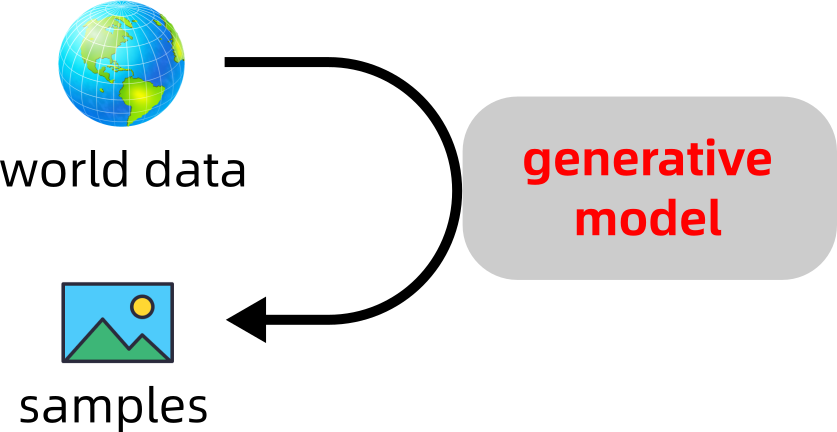
\includegraphics[scale=0.8]{generative-model.png}}}
\end{equation}
\textbf{LLMs} are a special case of generative models:
\begin{equation}
	\vcenter{\hbox{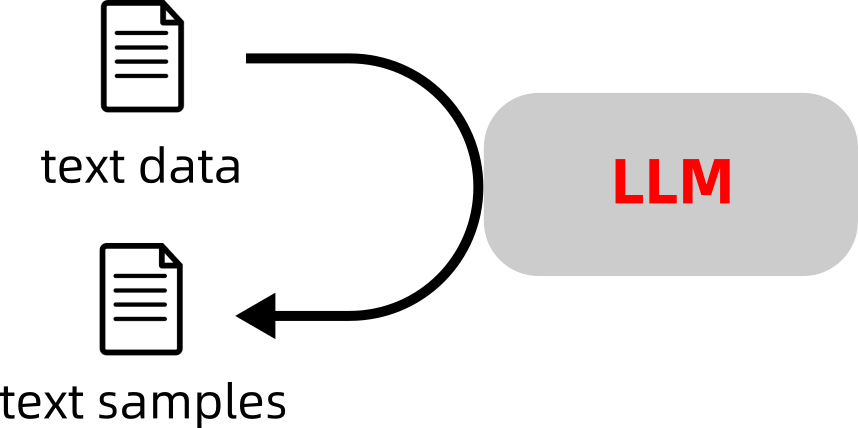
\includegraphics[scale=0.8]{LLM.png}}}
\end{equation}
One class of generative models are \textbf{auto-encoders}, which forces information to flow through a narrow bottleneck, thus \textbf{compressing} the data into a compact, latent representation:
\begin{equation}
	\vcenter{\hbox{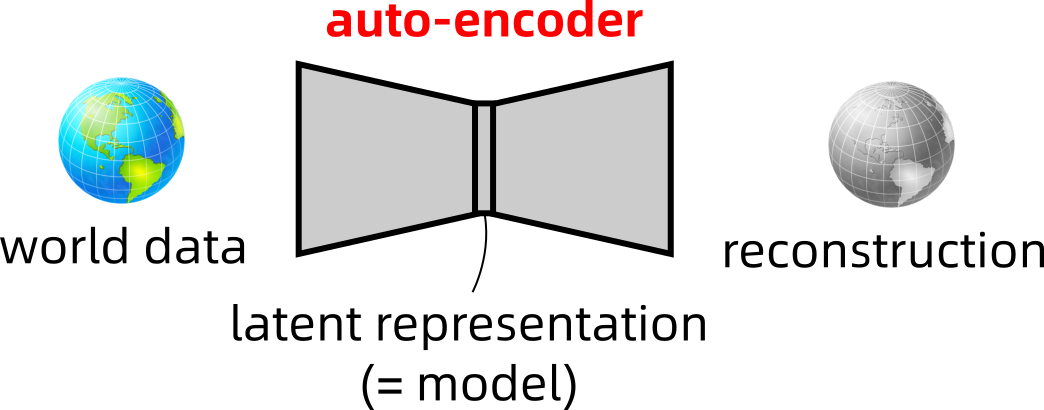
\includegraphics[scale=0.8]{auto-encoder.png}}}
	\label{fig:auto-encoder}
\end{equation}
Of which, the \textbf{VAE (variational auto-encoder)} uses variational methods to find a probability distribution $q_\phi(z|x)$ that approximates the true `posterior' distribution $q(z|x)$:
\begin{equation}
	\vcenter{\hbox{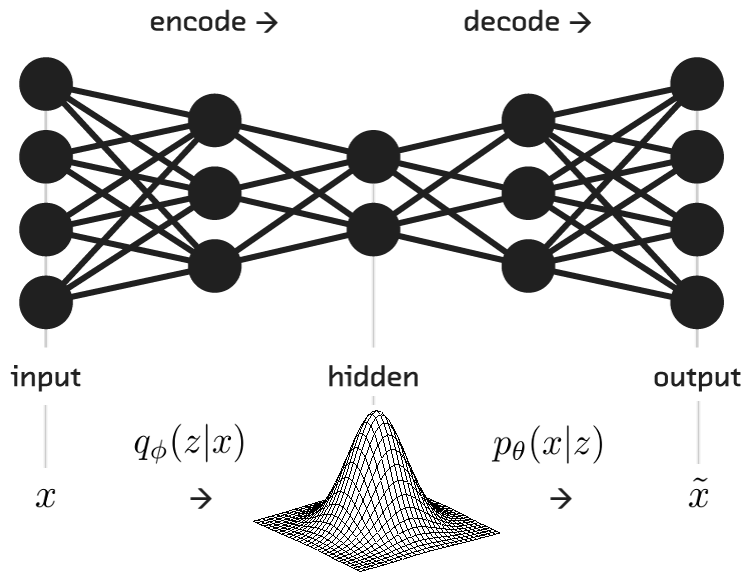
\includegraphics[scale=0.5]{VAE.png}}}
\end{equation}
One variational inference algorithm recently proposed is \textbf{SVGD (Stein variational gradient descent)} which exploits efficiency in reproducing kernel Hilbert space.

Another generative model is the \textbf{diffusion model}, whose latent representation is distributed among its many layers:
\begin{equation}
	\vcenter{\hbox{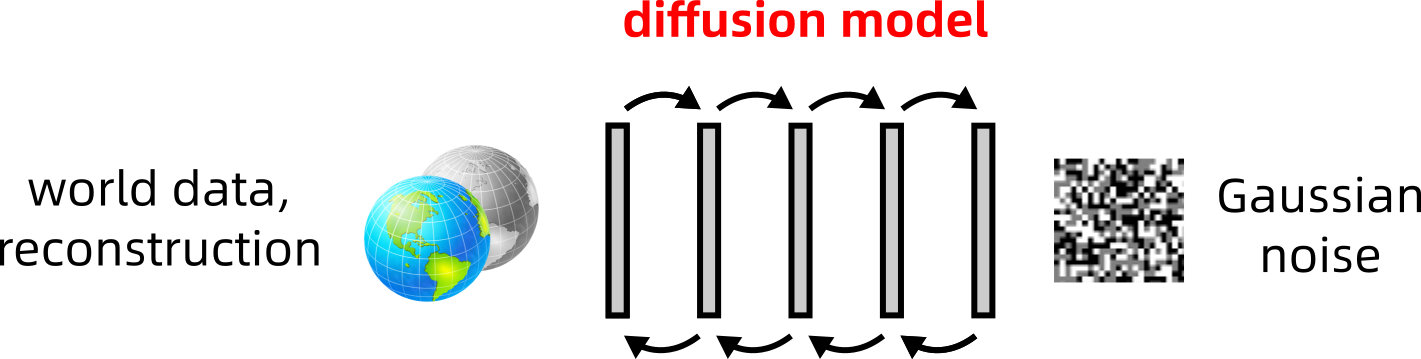
\includegraphics[scale=0.8]{diffusion-model.png}}}
\end{equation}

Interestingly, the \textbf{human brain} also has the structure of an auto-encoder.  Sensory information is processed by a hierarchy of cortical areas, getting increasingly abstract representations, which information is then \textbf{back-projected} towards the primary sensory areas, thus forming an auto-encoder similar to (\ref{fig:auto-encoder}) but folded in the middle.
\begin{equation}
	\vcenter{\hbox{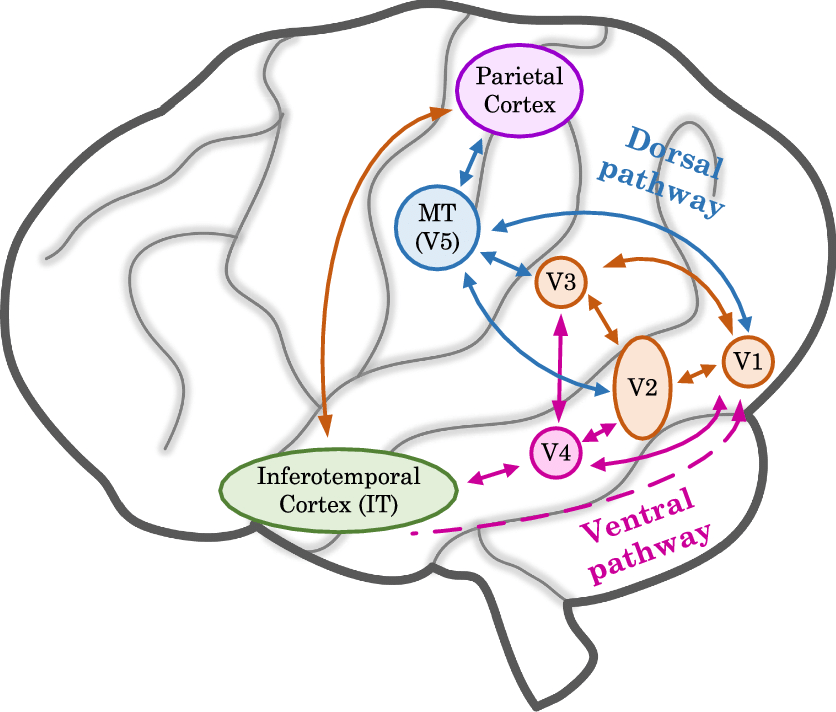
\includegraphics[scale=1.2]{visual-cortex.png}}}
\end{equation}


\end{minipage}
\end{preview}

\begin{preview}
\begin{textblock*}{5cm}(2.1cm,2.3cm) % {block width} (coords) 
	{\color{red}{\large \textcircled{\small \themypage}}}
	\addtocounter{mypage}{1}
\end{textblock*}

\begin{minipage}{\textwidth}
	\setlength{\parskip}{0.4\baselineskip}

\section{Reinforcement learning}

AGI should be developed under the framework of \textbf{RL (reinforcement learning)}, which tries to find an optimal policy that acts in an environment, that maximizes the total reward over a time horizon:
\begin{equation}
\vcenter{\hbox{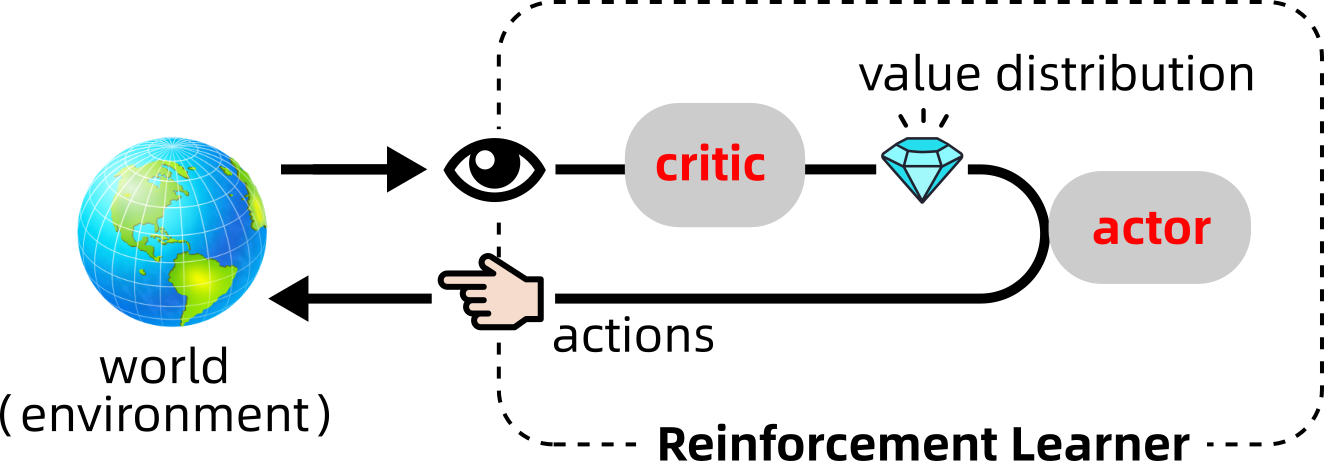
\includegraphics[scale=0.75]{RL.png}}}
\end{equation}

In its most general form, an RL algorithm tries to maximize the following Bellman objective:
\begin{equation}
\max_{\pi} \; \underset{\substack{a_t \;\sim\; \pi(\cdot | s_t) \\ s_{t+1} \;\sim\; p(\cdot | s_t, a_t) }} {\mathbb{E}} \left[ \sum_{t} \gamma^t R(s_t, a_t) \right]
\label{eqn:RL-objective}
\end{equation}
RL only needs to learn two things (probability distributions): the \textbf{policy} $\pi$ which is concerned with ``values'', and the \textbf{world model} $p$ which is concerned with ``truths''.

State-of-the-art RL algorithms tend to have an actor-critic structure, that simultaneously learns \textbf{value functions} (denoted $Q$ or $V$) and \textbf{policy functions} (denoted $\pi$).

I tend to favor the \textbf{SAC (soft actor-critic)} algorithm for AGI because it has an elegant theoretical underpinning based on entropy maximization.  If an RL algorithm always chooses the highest reward and does not explore the environment, such a strategy may turn out inferior to one that has some kind of ``curiosity''.  So we add an entropy term $H$ to the objective (\ref{eqn:RL-objective}) to make it ``soft'', so the agent tries to maximize rewards as well as make its behavior most ``random'':
\begin{equation}
\max_\pi \mathbb{E}_\pi \left[ \sum_t \gamma^t R(s_t, a_t) + \alpha H(\pi(a_t | s_t)) \right]
\label{eqn:SAC-objective}
\end{equation}

The function $Q(s,a)$ is a cross-section of the value function $V(s)$, which explicitly shows the choice of actions.  If we always choose $\argmax_a Q(s,a)$, such a strategy is purely exploitative.  So we make Q into a probability distribution via Boltzmann's construction:
\begin{equation}
\pi(\mathbf{a}|\mathbf{s}) \propto \frac{\exp Q(\mathbf{s}, \mathbf{a}) }{Z}
\end{equation}
where $Z$ is the partition function.  It turns out amazingly that this policy maximizes the objective (\ref{eqn:SAC-objective})

\section{RL + World Model}

The simplest RL architecture is like this:
\begin{equation}
\vcenter{\hbox{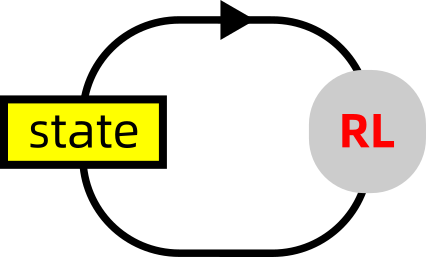
\includegraphics[scale=0.75]{minimal-RL.png}}}
\end{equation}
I propose to integrate it with an auto-encoder like this:
\begin{equation}
\vcenter{\hbox{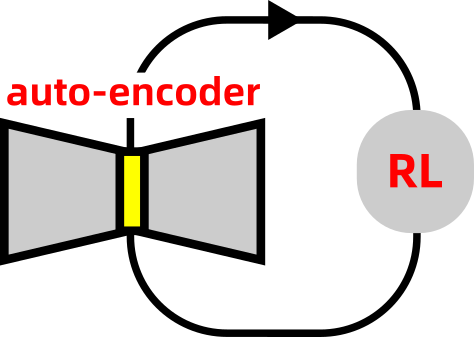
\includegraphics[scale=0.75]{RL-with-autoencoder.png}}}
\end{equation}
which means the two algorithms shares the same state.

For example, if the auto-encoder sees an apple then it produces a high-level representation of apple in its hidden layer(s).  If the RL desires to eat an apple it will produce the actions necessary to grab it.

One tricky issue here deserves explanation: I posited the RL to work in ``\textbf{mental space}'', whose actions are ``\textbf{thoughts}'' (but could also include real physical actions).  So the RL not only learns how to act in the world, but also learns how to ``think'' based on rewards.  After some thinking I concluded that this setup will not create inconsistencies.

Now the state (yellow box) is altered by two different algorithms with distinct objectives.  After some considerations I also tend to think it is OK....

\subsection{About our group}

We operate as a \textbf{DAO} (decentralized autonomous organization) based on transparent operations and reward system based on weighted voting, to enable global collaboration without racial (or other forms of) discrimination.

We value: democracy, freedom of speech, racial equality, transparency, tolerance of mistakes, and a learning environment.

It is OK for anyone to challenge other member's theories, ideas, proposals, etc.

%The actor and critic seem distinct from the world model.  The world model learns to predict the next state from the current state and action, ie. $p(s_{t+1} | s_t, a_t)$.  As such, it is not influenced by rewards or ``value judgements''.  We could say that the world model seeks only the ``\textbf{truth}'', whereas the actor-critic seeks values \footnote{but we can also let the world model predict rewards as well, in which case its role partly overlaps with the critic.}.  How might a world model help RL be more efficient?  Perhaps by letting the actor-critic explore the world model virtually:
%\begin{equation}
%	\vcenter{\hbox{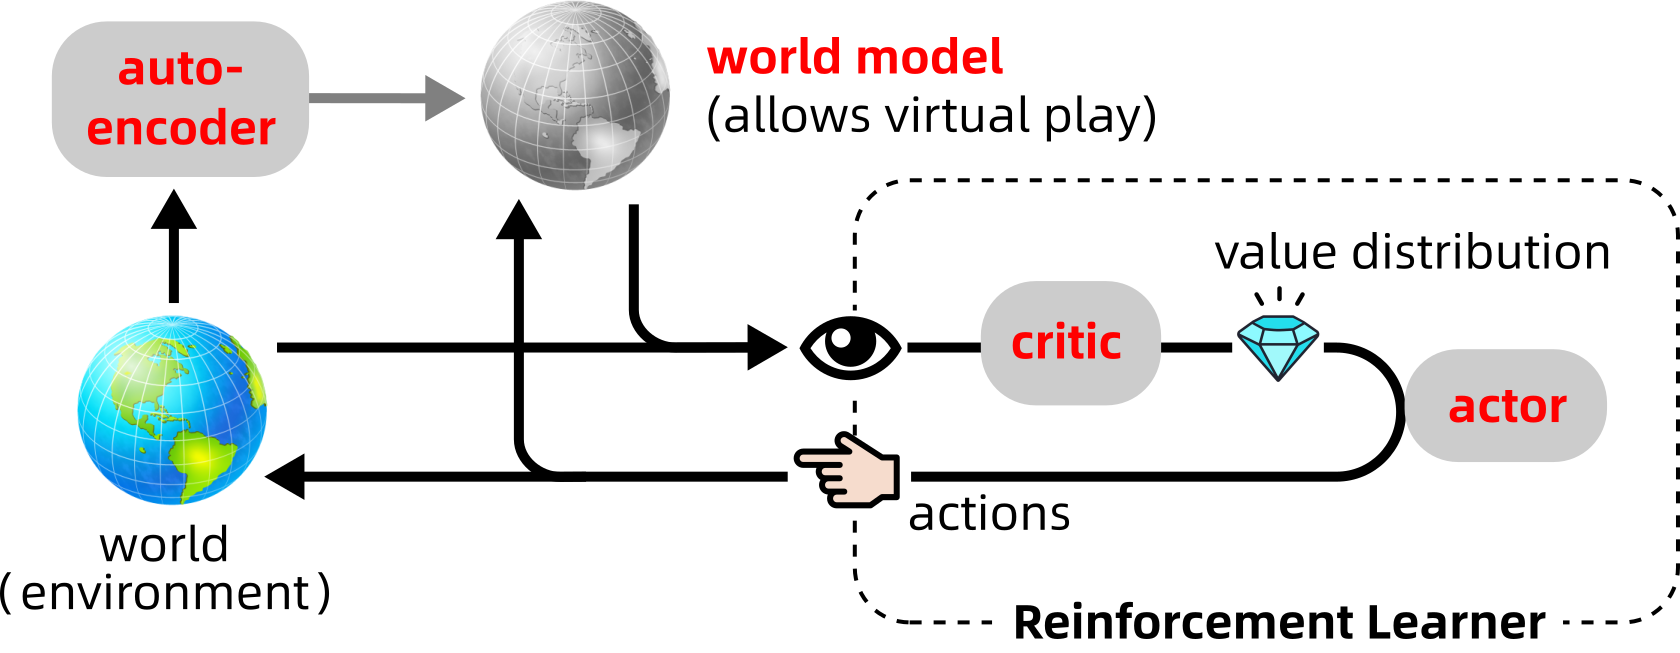
\includegraphics[scale=0.8]{RL-with-world-model.png}}}
%\end{equation}
%This is significant in physical environments, where physical actions are much more costly.  Ironically, most current AI training environments are already virtual, so this may not bring about large improvements.

\end{minipage}
\end{preview}

\begin{preview}
\begin{textblock*}{5cm}(2.1cm,2.3cm) % {block width} (coords) 
	{\color{red}{\large \textcircled{\small \themypage}}}
	\addtocounter{mypage}{1}
\end{textblock*}

\begin{minipage}{\textwidth}
	\setlength{\parskip}{0.4\baselineskip}

\section{Text world}

We want to find the ``path of least resistance'' to bootstrap an AGI.  Riding on the success of LLMs, we may want to train AGIs on a purely text-based environment.

An auto-encoder such as BERT would read a text and produce a latent representation (which could be in natural language, as NL is also a form of symbolic logic in a general sense).

The latent representation is the ``working memory'' of the intelligent system and its representation is more efficient for inferences than raw input.

The actor-critic of RL works in the latent representation (ie, a \textbf{model} of the world, taking virtual actions).  When a good virtual action is found, the algorithm would output an actual action.

\section{RL as ``thinking''}

Why take so much trouble to combine RL and LLM?  The benefit is that RL will find a way to optimize its internal ``thinking'' to achieve \textbf{logic coherence}.  This will cure the problem of LLM \textbf{hallucinations}.

This is feasible if we include ``thinking'' as ``\textbf{mental actions}'' in RL:
\begin{equation}
\vcenter{\hbox{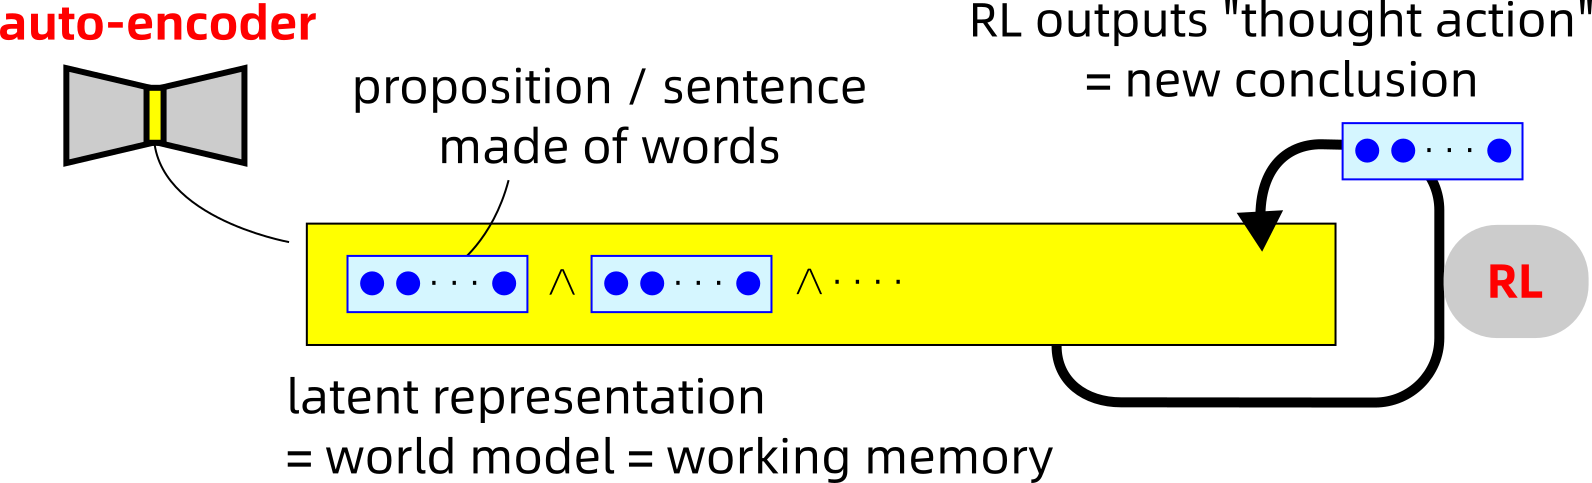
\includegraphics[scale=0.8]{RL-outputs-thought-action.png}}}
\end{equation}

\end{minipage}
\end{preview}

\end{document}
